\chapter{Double Integrals over Rectangular Regions}

fixme change intro to reflect shorter chapter
In this chapter, we extend this powerful idea into higher dimensions using the 
tools of multiple integration. While single integration enables us to calculate
the area under a curve or the volume under a surface, multiple integration 
allows us to calculate volumes in three dimensions, and even hypervolumes in 
higher dimensions.

We start by discussing double integration, which allows us to find the volume 
under a surface in three dimensions. This method involves slicing the solid 
into infinitesimally small columns, and summing the volumes of these columns.

Next, we'll cover triple integration, a tool that lets us find the volume of 
more complicated solids in three-dimensional space. The idea is similar to 
double integration.

To properly implement these techniques, we'll also discuss the different 
coordinate systems that can be used in multiple integration, such as 
rectangular, cylindrical, and spherical coordinates, and when it's advantageous
to use one system over another.

By the end of this chapter, you will have a deeper understanding of the 
techniques of multiple integration and how to apply them to find the volumes 
of various types of solids. The methods we study here will serve as a 
foundation for many topics in higher mathematics and physics, including 
electromagnetism, fluid dynamics, and quantum mechanics.

\section{Double Integrals}
Double integrals extend single-variable integration to functions of two 
variables, allowing us to calculate quantities like area, volume, and mass 
over a two-dimensional region. By integrating a function across a specified 
domain in the xy-plane, they help analyze how a quantity changes in both 
dimensions. Common in physics, engineering, and economics, double integrals 
involve setting up limits for the region and performing two successive 
integrations, often tailored to the region's geometry. We begin by discussing 
double integrals over rectangular regions, then extending that discussion to 
regions of any general shape. Finally, we discuss applications of double 
integrals. 

\subsection{Over Rectangular Regions}
Suppose there is some function, $z = f(x,y)$, that is defined over the 
rectangular region, \textit{R}, defined by $\textit{R} = [a, b] \times [c,d] = 
\{(x,y)| a \leq x \leq b, c \leq y \leq d\}$, and $f$ is such that $f \geq 0$ 
for all $(x, y) \in \mathbb{R}$. Then the graph of $f$ is a surface that lies 
above the rectangular region, \textit{R} (see figure \ref{fig:f_on_R}). 

\begin{figure}[htbp]
    \centering
    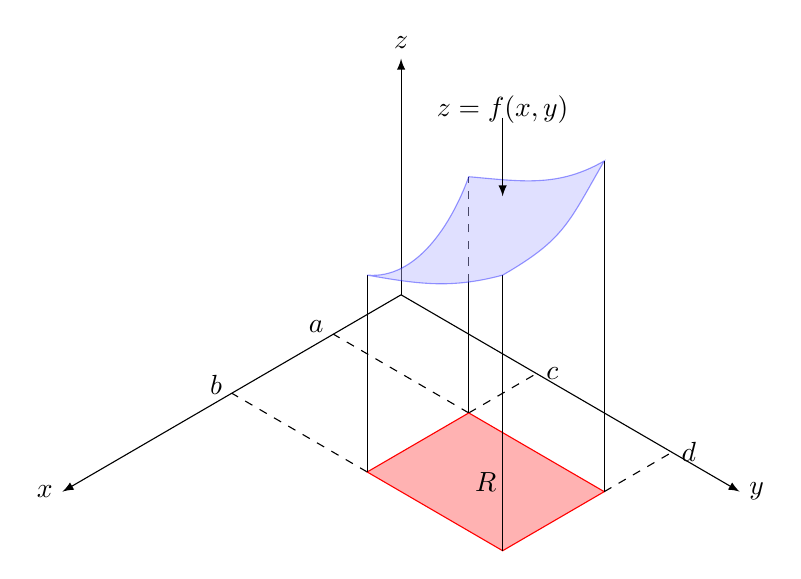
\begin{tikzpicture}[x = {(-0.86cm, -0.5cm)}, y = {(0.86cm, -0.5cm)}, 
    z = {(0cm, 1cm)}]
        \draw[-latex] (0,0,0) -- (5,0,0) node[left] {$x$};
        \draw[-latex] (0,0,0) -- (0,5,0) node[right] {$y$};
        \draw[-latex] (0,0,0) -- (0,0,3) node[above] {$z$};
        \draw[dashed] (1, 2, 0) -- (1, 0, 0) node[left, yshift = 0.1cm] {$a$};
        \draw[dashed] (2.5, 2, 0) -- (2.5, 0, 0) node[left, yshift = 0.1cm] 
        {$b$};
        \draw[dashed] (1, 2, 0) -- (0, 2, 0) node[right] {$c$};
        \draw[dashed] (1, 4, 0) -- (0, 4, 0) node[right] {$d$};
        \filldraw[draw = red, fill = red!30] (1, 2, 0) -- (2.5, 2, 0) -- 
        (2.5, 4, 0) -- (1, 4, 0) -- cycle;
        \node[] at (1.75, 3, 0) {$R$};
        \draw[] (2.5, 2, 0) -- (2.5, 2, 2.5);
        \draw[] (1, 2, 0) -- (1, 2, 1.66);
        \draw[dashed] (1, 2, 1.66) -- (1, 2, 3);
        \draw[] (2.5, 4, 0) -- (2.5, 4, 3.5);
        \draw[] (1, 4, 0) -- (1, 4, 4.2);
        \filldraw[draw = blue, fill = blue!30, opacity = 0.4] (2.5, 2, 2.5) 
        to[out = -5, in = -110, looseness = 0.9] (1, 2, 3) 
        to[out = -5, in = 210] (1, 4, 4.2) 
        to[out = 240, in = 30, looseness = 1.2] (2.5, 4, 3.5) 
        to[out = 195, in = -10] (2.5, 2, 2.5);
        \draw[-latex] (1, 2.5, 4) -- (1, 2.5, 3);
        \node[] at (1, 2.5, 4.1) {$z = f(x,y)$};
    \end{tikzpicture}
    \caption{The graph of $f$ over the region $R$}
    \label{fig:f_on_R}
\end{figure}

Let us call the solid that fills the space between the $xy$-plane and the 
surface $z = f(x,y)$ \textit{S}. Formally, this is written as
$$\textit{S} = \{ (x, y, z) \in \mathbb{R}^3 | 0 \leq z \leq f(x, y), (x, y) 
\in \mathbb{R}\}$$

How can we find the volume of the solid, \textit{S}? We will apply what we 
learned about Riemann sums and definite integrals in two dimensions to this 
three dimensional problem. 

First, we divide \textit{R} into rectangular subregions. We do this by 
dividing the interval $[a, b]$ into \textit{m} subintervals with width $\Delta 
x = (b - a)/m$ and the interval $[c, d]$ into \textit{n} subintervals with 
width $\Delta y = (d - c) / n$. Drawing lines through these divisions parallel 
to the $x$- and $y$-axes, we create a field of subrectangles, each with area 
$\Delta A = \Delta x \Delta y$ (see figure \ref{fig:subrectangles}). Each 
subrectangle is defined by:
$$\textit{R}_{ij} = [x_{i - 1}, x_i] \times [y_{j - 1}, y_j] - \{ (x, y) | x_{
i - 1} \leq x \leq x_i, y_{j - 1} \leq y \leq y_j \}$$ 

\begin{figure}[htbp]
    \centering
    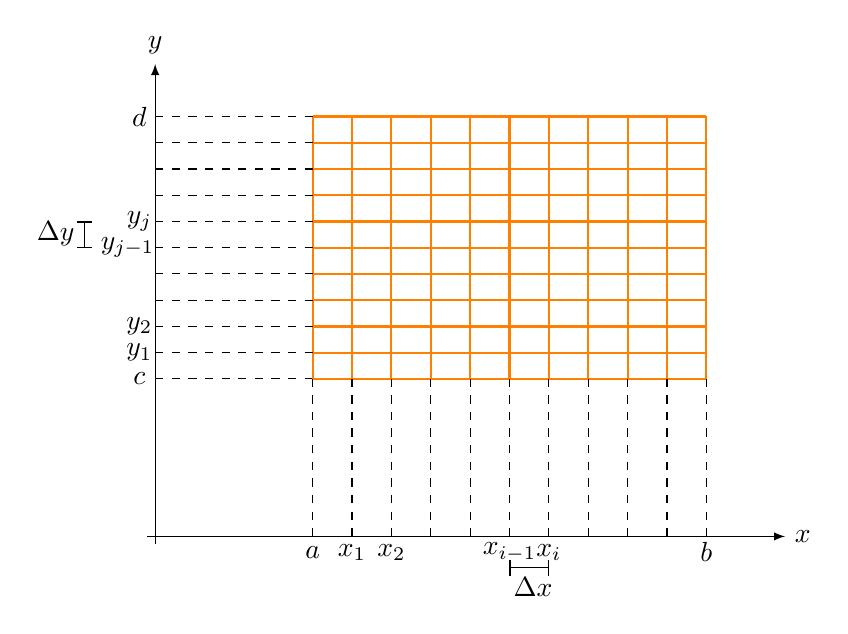
\begin{tikzpicture}
        \draw[-latex] (-0.1, 0) -- (8, 0) node[right] {$x$};
        \draw[-latex] (0, -0.1) -- (0, 6) node[above] {$y$};
        \foreach \i in {0,1, 2, 3, 4, 5, 6, 7, 8, 9, 10} {
            \draw[dashed] (2 + \i/2, 0) -- (2 + \i/2, 2);
            \draw[dashed] (0, 2 + \i/3) -- (2, 2 + \i/3);
            \draw[orange, thick] (2 + \i/2, 2) -- (2 + \i/2, 5.333);
            \draw[orange, thick] (2, 2 + \i/3) -- (7, 2 + \i/3);
            }
        \node[] at (2, -0.2) {$a$};
        \node[] at (7, -0.2) {$b$};
        \node[] at (2.5, -0.2) {$x_1$};
        \node[] at (3, -0.2) {$x_2$};
        \node[] at (4.5, -0.2) {$x_{i - 1}$};
        \node[] at (5, -0.2) {$x_i$};
        \draw[|-|] (4.5, -0.4) -- (5, -0.4) node[below, xshift = -0.2cm] 
        {$\Delta x$};
        \node[] at (-0.2, 2) {$c$};
        \node[] at (-0.2, 5.333) {$d$};
        \node[] at (-0.2, 2.333) {$y_1$};
        \node[] at (-0.2, 2.667) {$y_2$};
        \node[] at (-0.35, 3.667) {$y_{j - 1}$};
        \node[] at (-0.2, 4) {$y_j$};
        \draw[|-|] (-0.9, 3.667) -- (-0.9, 4) node[left, yshift = -0.15cm] 
        {$\Delta y$};
    \end{tikzpicture}
    \caption{The region, \textit{R}, on the $xy$-plane divided into 
    subrectangles}
    \label{fig:subrectangles}
\end{figure}

Since $f(x,y)$ in continuous over the \textit{R}, there is some point, $(x_{ij}
^*, y_{ij}^*)$, equal to the average value of $f(x,y)$ over the subrectangle. 
Then we can approximate the volume between the $xy$-plane and $z = f(x,y)$ over
the subrectangle as a column with base area $\Delta A$ and height $f(x_{ij}^*, 
y_{ij}^*)$ (seefigure \ref{fig:one_column}) and the volume of the column is 
given by:
$$V_{ij} = f(x_{ij}^*, y_{ij}^*) \Delta A$$

\begin{figure}[htbp]
    \centering
    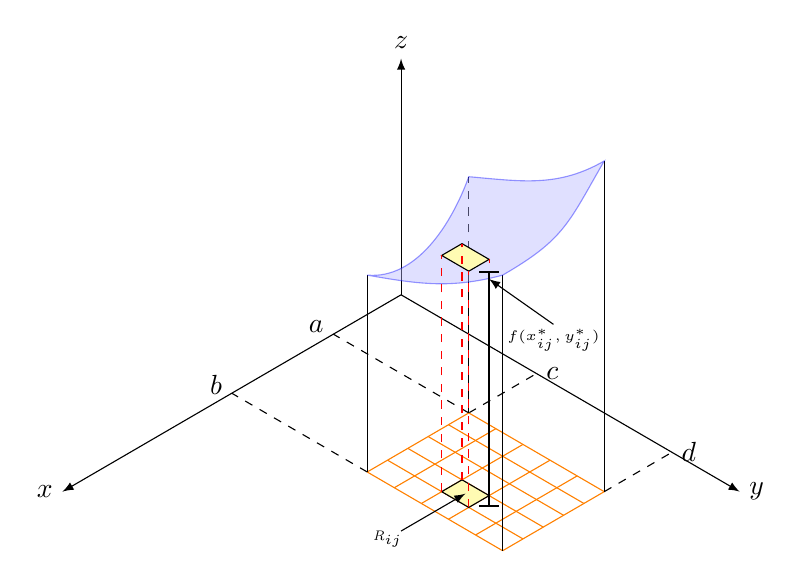
\begin{tikzpicture}[x = {(-0.86cm, -0.5cm)}, y = {(0.86cm, -0.5cm)}, 
    z = {(0cm, 1cm)}]
        \draw[-latex] (0,0,0) -- (5,0,0) node[left] {$x$};
        \draw[-latex] (0,0,0) -- (0,5,0) node[right] {$y$};
        \draw[-latex] (0,0,0) -- (0,0,3) node[above] {$z$};
        \draw[dashed] (1, 2, 0) -- (1, 0, 0) node[left, yshift = 0.1cm] {$a$};
        \draw[dashed] (2.5, 2, 0) -- (2.5, 0, 0) node[left, yshift = 0.1cm] 
        {$b$};
        \draw[dashed] (1, 2, 0) -- (0, 2, 0) node[right] {$c$};
        \draw[dashed] (1, 4, 0) -- (0, 4, 0) node[right] {$d$};
        \foreach \i in {0, 1, 2, 3, 4, 5} {
            \draw[orange] (1 + \i*1.5/5, 2, 0) -- (1 + \i*1.5/5, 4, 0);
            \draw[orange] (1, 2 + 2*\i/5, 0) -- (2.5, 2 + 2*\i/5, 0);
        }
        \draw[] (2.5, 2, 0) -- (2.5, 2, 2.5);
        \draw[] (1, 2, 0) -- (1, 2, 1.66);
        \draw[dashed] (1, 2, 1.66) -- (1, 2, 3);
        \draw[] (2.5, 4, 0) -- (2.5, 4, 3.5);
        \draw[] (1, 4, 0) -- (1, 4, 4.2);
        \filldraw[draw = blue, fill = blue!30, opacity = 0.4] (2.5, 2, 2.5) 
        to[out = -5, in = -110, looseness = 0.9] (1, 2, 3) 
        to[out = -5, in = 210] (1, 4, 4.2) 
        to[out = 240, in = 30, looseness = 1.2] (2.5, 4, 3.5) 
        to[out = 195, in = -10] (2.5, 2, 2.5);
        \filldraw[draw = black, fill = yellow!30] (1.9, 2.8, 0) -- 
        (1.9, 3.2, 0) -- (2.2, 3.2, 0) -- (2.2, 2.8, 0) -- cycle;
        \filldraw[draw = black, fill = yellow!30] (1.9, 2.8, 3) -- 
        (1.9, 3.2, 3) -- (2.2, 3.2, 3) -- (2.2, 2.8, 3) -- cycle;
        \foreach \x/\y in {1.9/2.8, 1.9/3.2, 2.2/3.2, 2.2/2.8} {
            \draw[red, dashed] (\x, \y, 0) -- (\x, \y, 3);
        }
        \draw[|-|, thick] (2.05, 3.35, 0) -- (2.05, 3.35, 3);
        \node[font = \tiny] at (0.75, 3, 1.3) {$f(x_{ij}^*, y_{ij}^*)$};
        \draw[-latex] (0.75, 3, 1.5) -- (2.05, 3.35, 2.9);
        \draw[-latex] (3, 3, 0) -- ( 2.05, 3, 0);
        \node[font = \tiny] at (3.2, 3, 0) {$\textit{R}_{ij}$};
    \end{tikzpicture}
    \caption{A single column with base $\Delta A$ and height $f(x_{ij}^*, 
    y_{ij}^*)$}
    \label{fig:one_column}
\end{figure}

And therefore the approximate volume of the solid, \textit{S}, that lies 
between the region, \textit{R}, and $z = f(x,y)$ is the sum of all the columns 
over $i$ and $j$:
$$V_{\textit{S}} \approx \sum_{i = 1}^n \sum_{j = 1}^n f(x_{ij}^*, y_{ij}^*) 
\Delta A$$

And just like with the area under a curve, we get the true volume by taking the
limit as $n \to \infty$, which becomes a \textbf{double integral}\index{double 
integral}:

\begin{mdframed}[style = important, frametitle = {Volume of a Solid over a 
Region}]
$$V_{\textit{S}} = \lim_{n \to \infty} \sum_{i = 1}^n \sum_{j = 1}^n f(x_{ij}^*
, y_{ij}^*) \Delta A = \iint_{\textit{R}} f(x, y)\,dA$$
\end{mdframed}


\section{Iterated Integrals}

To be able to evaluate the double integral as outlined above, we must first 
discuss iterated integrals. Iterated integrals happen when you evaluate two 
single integrals, one inside the other. Consider some function, $g(x, y)$. We 
could integrate that function from $x = q$ to $x = r$ thusly:
$$\int_q^r g(x, y)\,dx$$
Notice that we are integrating with respect to $x$, so $y$ terms will be 
treated as constants (recall partial differentiation: this is the opposite 
process). Let's call the result of this first integral $A(y)$:
$$A(y) = \int_q^r g(x, y)\,dx$$

We can then integrate the resulting function, $A(y)$, from $y = s$ to $y = t$:
$$\int_s^t A(y)\,dy = \int_s^t \left[ \int_q^r g(x, y)\,dx \right]\,dy$$
This is called an \textbf{iterated integral}\index{iterated integral}. When 
evaluating iterated integrals, we work from the inside out. You can also write 
it without the brackets:
$$\int_s^t \int_q^r g(x, y)\,dx\,dy$$

\textbf{Example}: evaluate the iterated integral $\int_0^3 \int_1^2 x y^2\,dy
\,dx$.

\textbf{Solution}: We can re-write this to more explicitly show the inner and 
outer integrals:
$$\int_0^3 \left[ \int_1^2 x y^2\,dy \right]\,dx$$
As you can see, the inner integral is with respect to $y$. Let's isolate and 
evaluate the inner integral:
$$\int_1^2 x y^2\,dy = x \int_1^2 y^2\,dy = x \left[ \frac{1}{3}y^2 \right]_{y 
= 1}^{y = 2}$$
$$= \frac{x}{3} \left[ 2^3 - 1^3 \right] = \frac{x}{3} \left[ 8 - 1 \right] = 
\frac{7x}{3}$$

We were able to move $x$ outside the integral because when we are integrating 
with respect to a specific variable (in this case, $y$), other variables are 
treated as constants. Now we can substitute $\int_1^2 xy^2 \,dy = \frac{7x}{3}$
into the iterated integral:
$$\int_0^3 \left[ \int_1^2 x y^2\,dy \right]\,dx = \int_0^3 \left[ \frac{7x}{3}
\right]\,dx$$
$$= \frac{7}{3} \left[ \frac{1}{2}x^2 \right]_{x = 0}^{x = 3} = \frac{7}{6} 
\left[ 3^2 - 0^2 \right] = \frac{7 \cdot 9}{6} = \frac{21}{2}$$

\begin{Exercise}[title = {Order of Evaluating Iterated Integrals}, label = 
iterate 1]
Show that $\int_0^3 \int_1^2 x y^2\,dy\,dx = \int_1^2 \int_0^3 x y^2 \,dx\,dy$.
\end{Exercise}

\begin{Answer}[ref = iterate_1]
We have already shown that $\int_0^3 \int_1^2 x y^2\,dy\,dx = \frac{21}{2}$. 
We will evaluate $\int_1^2 \int_0^3 x y^2 \,dx\,dy$ and see if we get the same 
result. 
$$\int_0^3 x y^2 \,dx = y^2 \int_0^3 x\,dx = y^2 \left[ \frac{1}{2}x^2 \right]_
{x = 0}^{x = 3}$$
$$= \frac{y^2}{2} \left[ 3^2 - 0^2 \right] = \frac{9y^2}{2}$$
Substituting this back into the iterated integral:
$$\int_1^2 \int_0^3 x y^2 \,dx\,dy = \int_1^2 \frac{9y^2}{2}\,dy = \frac{9}{2} 
\int_1^2 y^2 \,dy$$
$$= \frac{9}{2} \left[ \frac{1}{3}y^3 \right]_{y = 1}^{y = 2} = \frac{9}{2} 
\cdot \frac{1}{3} \left[ 2^3 - 1^3 \right]$$
$$= \frac{3}{2}(8 - 1) = \frac{21}{2}$$
\end{Answer}

\begin{Exercise}[title = {Evaluating Iterated Integrals}, label = iterate_2]
Evaluate the following iterated integrals.
\begin{enumerate}
\item $\int_0^1 \int_1^2 \left( x + e^{-y} \right)\,dx\,dy$
\item $\int_{-3}^3 \int_{0}^{\pi/2} \left( 2y + y^2 \cos{x} \right)\,dx\,dy$
\item $\int_0^3 \int_0^{\pi/2} t^2 \sin^3{\theta}\,d\theta\,dt$
\end{enumerate}
\vspace{100mm}
\end{Exercise}

\begin{Answer}[ref = iterate_2]
\begin{enumerate}
\item Answer: $\frac{5}{2} - \frac{1}{e}$. Solution: $\int_0^1 \int_1^2 \left( 
x + e^{-y} \right)\,dx\,dy = \int_0^1 \left( \frac{1}{2}x^2 + xe^{-y} \right)
|_{x=1}^{x=2}\,dy = \int_0^1 \left( 2 - \frac{1}{2} + 2e^{-y} - e^{-y} \right)
\,dy = \int_0^1 \left( \frac{3}{2} + e^{-y} \right)\,dy = \left[ \frac{3}{2}y 
- e^{-y} \right]_{y = 0}^{y = 1} = \left( \frac{3}{2}(1) - e^{-1} \right) - 
\left( \frac{3}{2}(0) - e^0 \right) = \frac{5}{2} - \frac{1}{e}$
\item Answer: $18$. Solution: $\int_{-3}^3 \int_{0}^{\pi/2} \left( 2y + y^2 
\cos{x} \right)\,dx\,dy = \int_{-3}^3 \left[ 2xy + y^2 \sin{x} \right]_{x = 0}^
{x = \pi/2}\,dy = \int_{-3}^3 \left[ \left( \pi y + y^2 \right) - \left( 0 + 0 
\right) \right]\,dy = \int_{-3}^3 \left( \pi y + y^2 \right)\,dy = \left[ 
\frac{\pi}{2}y^2 + \frac{1}{3}y^3 \right]_{y = -3}^{y = 3} = \left( \frac{\pi}{
2}(9) + \frac{1}{3}(27) \right) - \left( \frac{\pi}{2}(9) + \frac{1}{3}(-27) 
\right) = 9 - (-9) = 18$
\item Answer: $6$. Solution: $\int_0^3 \int_0^{\pi/2} t^2 \sin^3{\theta}\,
d\theta\,dt = \left( \int_0^3 t^2\,dt \right) \times \left( \int_0^{\pi/2} 
\sin^3{\theta}\,d\theta \right) = \left[ \frac{1}{3}t^3 \right]_{t = 0}^{t = 3}
\times \left( \int_0^{\pi/2} \sin{\theta} \sin^2{\theta}\,d\theta \right) = 9
\int_0^{\pi/2} \sin{\theta} \left( 1 - \cos^2{\theta} \right)\,d\theta = 9 
\left[ \int_0^{\pi/2} \sin{\theta}\,d\theta - \int_0^{\pi/2} \sin{\theta}
\cos^2{\theta}\,d\theta \right] = 9 \left[ \left( -\cos{\theta} \right) |_{
\theta = 0}^{\theta = \pi/2} + \left( \frac{1}{3}\cos^3{\theta} \right)|_{
\theta = 0}^{\theta = \pi/2} \right] = 9 \left[ -(-\cos{0}) + (-\frac{1}{3}
\cos^3{0}) \right] = 9 \left( 1 - \frac{1}{3} \right) = 9 \left( \frac{2}{3} 
\right) = 6$
\end{enumerate}
\end{Answer}

\section{Fubini's Theorem for Double Integrals}

Fubini's theorem states that for a 
function, $f$, that is continuous over the rectangular region, \textit{R}, the 
double integral of $f$ over the region $\textit{R} = \{ (x, y) | a \leq x \leq 
b, c \leq y \leq d\}$ is equal to the iterated integral of $f$ with respect to 
$x$ and $y$. This is expressed mathematically below:

\begin{mdframed}[style = important, frametitle = {Fubini's Theorem}]
If $f$ is continuous on the rectangle $R = \{ \left( x, y \right) | a \leq x 
\leq b, c \leq y \leq d \}$, then
$$\iint_R f(x,y)\,\,dA = \int_a^b \int_c^d f(x,y)\,dy\,dx = \int_c^d \int_a^b 
f(x,y)\,dx\,dy$$
\end{mdframed}

\begin{Exercise}[title={Applying Fubini's Theorem},label = fubini_1]
Rewrite the following double integrals as iterated integrals.
\begin{enumerate}
\item $\iint_R \frac{xy^2}{x^2 + 1}\,\,dA$, $R = \{(x,y)|0 \leq x \leq 1, -3 
\leq y \leq 3\}$
\item $\iint_R \frac{\sec{\theta}}{\sqrt{1 + t^2}}\,\,dA$, $R = \{(\theta, t) |
0 \leq \theta \leq \frac{\pi}{4}, 0 \leq t \leq 1 \}$
\end{enumerate}
\vspace{40mm}
\end{Exercise}

\begin{Answer}[ref = fubini_1]
\begin{enumerate}
\item $\int_0^1 \int_{-3}^3 \frac{xy^2}{x^2 + 1}\,dy\,dx$ OR $\int_{-3}^3 
\int_0^1 \frac{xy^2}{x^2 + 1}\,dx\,dy$
\item $\int_0^{\pi/4} \int_0^1 \frac{\sec{\theta}}{\sqrt{1 + t^2}}\,dt\,
d\theta$ OR $\int_0^1 \int_0^{\pi/4} \frac{\sec{\theta}}{\sqrt{1 + t^2}}\,
d\theta \,dt$
\end{enumerate}
\end{Answer}

\begin{Exercise}[label = fubini_2]
Evaluate the double integral. 
\begin{enumerate}
\item $\iint_R \frac{xy^2}{x^2 + 1}\,dA$, $\textit{R} = \{ \left( x, y \right) 
| \text{ } 0 \leq x \leq 2, \text{ } -3 \leq y \leq 3 \}$
\item $\iint_R \frac{\tan{\theta}}{\sqrt{1 - t^2}}\,dA$, $\textit{R} = \{ 
\left( \theta, t \right) | \text{ } 0 \leq \theta \leq \pi/3, \text{ } 0 \leq 
t \leq \frac{1}{2} \}$
\item $\iint_R x \sin{ \left( x + y \right) }\,dA$, $\textit{R} = \left[0, 
\pi/6 \right] \times \left[ 0, \pi/3 \right]$
\end{enumerate}
\end{Exercise}

\begin{Answer}[ref = fubini_2]
\begin{enumerate}
\item $\iint_R \frac{xy^2}{x^2 + 1}\,dA$, $\textit{R} = \{ \left( x, y \right) 
| 0 \leq x \leq 2, -3 \leq y \leq 3 \} = \int_0^2 \int_{-3}^3 \frac{xy^2}{x^2 
+ 1}\,dy\,dx = \int_0^2 \frac{x}{x^2 + 1}\,dx \cdot \int_{-3}^{3} y^2\,dy$. To 
evaluate the integral with respect to $x$, we use the $u$-substitution $u = 
x^2 + 1$, $(x)dx = \frac{1}{2} du$: $\int_0^2 \frac{x}{x^2 + 1}\,dx \cdot 
\int_{-3}^{3} y^2\,dy = \int_{x = 0}^{x = 2} \frac{1}{2} \frac{1}{u}\,du \cdot 
\int_{-3}^3 y^2\,dy = \frac{1}{2} \ln{|u|}|_{x = 0}^{x = 2} \cdot \frac{1}{3} 
\left[ y^3 \right]_{y = -3}^{y = 3} = \frac{1}{2} \left[ \ln{\left( 2^2 + 1 
\right) - \ln{ \left( 0^2 + 1 \right)}} \right] \cdot \frac{1}{3} \left[ 3^3 - 
\left( -3 \right)^3 \right] = \frac{1}{2} \ln{5} \cdot \frac{1}{3} \left( 27 - 
(-27) \right) = \frac{\ln{5}}{2} \frac{54}{3} = 9\ln{5}$
\item $\iint_R \frac{\tan{\theta}}{\sqrt{1 - t^2}}\,dA$, $\textit{R} = \{ 
\left( \theta, t \right) | \text{ } 0 \leq \theta \leq \pi/3, \text{ } 0 \leq 
t \leq \frac{1}{2} \} = \int_0^{\pi/3} \int_0^{1/2} \frac{\tan{\theta}}{\sqrt{
1 - t^2}}\,dt\,d\theta = \left[ \int_0^{\pi/3} \tan{\theta}\,d\theta \right] 
\cdot \left[ \int_0^{1/2} \frac{1}{\sqrt{1 - t^2}}\,dt \right]$. Recall that 
$\frac{d}{dt} \arcsin{t} = \frac{1}{\sqrt{1 - t^2}}$. Applying FTC, then 
$\left[ \int_0^{\pi/3} \tan{\theta}\,d\theta \right] \cdot \left[ \int_0^{1/2} 
\frac{1}{\sqrt{1 - t^2}}\,dt \right] = \left[ \int_0^{\pi/3} \tan{\theta}\,d\theta 
\right] \cdot \left[ \arcsin{t} \right]_{t = 0}^{t = 1/2} = \left[ \int_0^{\pi/
3} \tan{\theta}\,d\theta \right] \cdot \left[ \arcsin{\frac{1}{2}} - \arcsin{0}
\right] = \left[ \int_0^{\pi/3} \tan{\theta}\,d\theta \right] \cdot \left[ 
\frac{\pi}{6} \right] = \frac{\pi}{6} \int_0^{\pi/3} \frac{\sin{\theta}}{\cos{
\theta}}\,d\theta$. To evaluate this final integral, we use the $u$-substitution
$u = \cos{\theta}$ and $-du = \sin{\theta} d\theta$: $\frac{\pi}{6} \int_0^{\pi
/3} \frac{\sin{\theta}}{\cos{\theta}}\,d\theta = -\frac{\pi}{6}\int_{\theta = 0
}^{\theta = \pi/3} \frac{1}{u}\,du = -\frac{\pi}{6} \ln{u}|_{\theta = 0}^{
\theta = \pi/3} = -\frac{\pi}{6} \left[ \ln{ \left( \cos{\theta} \right)} 
\right]_{\theta = o}^{\theta = \pi/3} = \frac{\pi}{6} \left[ \ln{\left( \cos{0} 
\right) - \ln{ \left( \cos{\frac{\pi}{3}} \right)}} \right] = \frac{\pi}{6} 
\left[ \ln{1} - \ln{\frac{1}{2}} \right] = \frac{\pi}{6} \ln{\frac{1}{1/2}} = 
\frac{\pi}{6} \ln{2}$
\item $\iint_R x \sin{ \left( x + y \right) }\,dA$, $\textit{R} = \left[0, 
\pi/6 \right] \times \left[ 0, \pi/3 \right] = \int_0^{\pi/6} \int_0^{\pi/3} x 
\sin{ \left( x + y \right) }\,dy\,dx$. Recall the sum formula for sine:
$$\sin{ \left( x + y \right)} = \sin{x}\cos{y} + \cos{x}\sin{y}$$

We can substitute this into our iterated integral:
$$\int_0^{\pi/6} \int_0^{\pi/3} x \sin{ \left( x + y \right) }\,dy\,dx = 
\int_0^{\pi/6} \int_0^{\pi/3} x \left[ \sin{x}\cos{y} + \cos{x}\sin{y} 
\right]\,dy\,dx$$
$$= \int_0^{\pi/6} \left[ \int_0^{\pi/3} x \sin{x} \cos{y}\,dy + \int_0^{\pi/3}
x \cos{x} \sin{y}\,dy \right]\,dx$$

Let us designate $\int_0^{\pi/3} x \sin{x} \cos{y}\,dy$ as integral \textbf{A} 
and $\int_0^{\pi/3} x \cos{x} \sin{y}\,dy$ as integral \textbf{B}. First, we 
will evaluate integral \textbf{A}:
$$\int_0^{\pi/3} x \sin{x} \cos{y}\,dy = x \sin{x} \int_0^{\pi/3} \cos{y}\,dy$$
$$= x \sin{x} \left[ \sin{y} \right]_{y = 0}^{y = \pi/3} = x \sin{x} \left[ 
\sin{\frac{\pi}{3}} - \sin{0} \right]$$
$$= x \sin{x} \left( \frac{\sqrt{3}}{2} \right) = \frac{x \sqrt{3}}{2} \sin{x}$$

Next we evaluate integral \textbf{B}:
$$\int_0^{\pi/3} x \cos{x} \sin{y}\,dy = x \cos{x} \int_0^{\pi/3} \sin{y}\,dy$$
$$= x \cos{x} \left[ - \cos{y} \right]_{y = 0}^{y = \pi/3} = x \cos{x} \left[ -
\cos{\frac{\pi}{3}} - \left( - \cos{0} \right) \right]$$
$$= x\cos{x} \left[ - \frac{1}{2} - (-1) \right] = \frac{x}{2}\cos{x}$$

Substituting back in for integrals \textbf{A} and \textbf{B}:
$$\int_0^{\pi/6} \left[ \int_0^{\pi/3} x \sin{x} \cos{y}\,dy + \int_0^{\pi/3} 
x \cos{x} \sin{y}\,dy \right]\,dx = \int_0^{\pi/6} \left[ \frac{x \sqrt{3}}{2} 
\sin{x} + \frac{x}{2}\cos{x} \right]\,dx$$
$$= \frac{\sqrt{3}}{2} \int_0^{\pi/6} x \sin{x}\,dx + \frac{1}{2} \int_0^{
\pi/6} x \cos{x}\,dx$$

Again, we will designate $\int_0^{\pi/6} x \sin{x}\,dx$ as integral \textbf{C} 
and $\int_0^{\pi/6} x \cos{x}\,dx$ as integral \textbf{D}. We start by using 
integration by parts to evaluate integral \textbf{C}:

Let $u = x$ and $dv = \sin{x} dx$. Then $v = -cos{x}$ and $du = dx$ and 
therefore:
$$\int_0^{\pi/6} x \sin{x}\,dx = \left[ x \left(- \cos{x} \right) \right]_{x = 
0}^{x = \pi/6} - \int_0^{\pi/6} \left( - \cos{x} \right)\,dx$$
$$= \left[ \frac{\pi}{6} \left(- \cos{\frac{\pi}{6}} \right) \right] - \left[ 
0 \left(- \cos{0} \right) \right] + \sin{x}|_{x = 0}^{x = \pi/6}$$
$$= -\frac{\pi}{6} \cdot \frac{\sqrt{3}}{2} - 0 + \sin{\frac{\pi}{6}} - 
\sin{0} = \frac{1}{2} - \frac{\pi \sqrt{3}}{12} = \frac{6 - \pi \sqrt{3}}{12}$$

Next, we will use integration by parts to evaluate integral \textbf{D}. Let $u 
= x$ and $dv = \cos{x} dx$. Then $du = dx$ and $v = \sin{x}$ and therefore:
$$\int_0^{\pi/6} x \cos{x}\,dx = \left[ x \sin{x} \right]_{x = 0}^{x = \pi/6} -
\int_0^{\pi/6} \sin{x}\,dx$$
$$= \left[ \frac{\pi}{6}\sin{\frac{\pi}{6}} - 0\sin{0} \right] - \left( - 
\cos{x} \right)|_{x = 0}^{x = \pi/6} = \frac{\pi}{6} \cdot \frac{1}{2} + 
\cos{\frac{\pi}{6}} - \cos{0}$$
$$= \frac{\pi}{12} + \frac{\sqrt{3}}{2} - 1 = \frac{\pi + 6\sqrt{3} - 12}{12}$$

Substituting back in for integrals \textbf{C} and \textbf{D}:
$$\frac{\sqrt{3}}{2} \int_0^{\pi/6} x \sin{x}\,dx + \frac{1}{2} \int_0^{\pi/6} 
x \cos{x}\,dx = \frac{\sqrt{3}}{2} \left( \frac{6 - \pi \sqrt{3}}{12} \right) 
+ \frac{1}{2} \left( \frac{\pi + 6\sqrt{3}- 12}{12} \right)$$
$$= \frac{6 \sqrt{3} - 3\pi + \pi + 6\sqrt{3} - 12}{24} = \frac{6 \sqrt{3} - 6 
- \pi}{12}$$
\end{enumerate}
\end{Answer}



